% =====================================================================
%  Section 8.4: Godunov's method.
% =====================================================================

\subsection{Godunov's method}
\label{subsec:godunov}

\subsubsection{The scheme}
\label{subsubsec:godunov-flux}

Let $\mathbb{R}$ be divided into cells $[x_{j-1/2},x_{j+1/2}]$ of width
$\Delta x$, with $t^n=n\Delta t$ and cell averages
$\bar u_j^n=\Delta x^{-1}\int_{x_{j-1/2}}^{x_{j+1/2}}u(x,t^n)\,dx$ approximated by $U_j^n$.
Integrating $u_t+f(u)_x=0$ over a cell and a time step gives
\begin{equation}
  \bar u_j^{n+1} = \bar u_j^n - \frac{\Delta t}{\Delta x}
  \left( F_{j+1/2}^n - F_{j-1/2}^n \right),
  \qquad F_{j+1/2}^n=\frac1{\Delta t}\int_{t^n}^{t^{n+1}}f\big(u(x_{j+1/2},t)\big)\,dt,
\end{equation}
for the exact cell averages $\bar u_j^n$. The scheme replaces $F_{j+1/2}^n$ by a
numerical flux $\widehat f_{j+1/2}$ depending on $U_j^n,U_{j+1}^n$, giving
$U_j^{n+1}=U_j^n-\frac{\Delta t}{\Delta x}(\widehat f_{j+1/2}-\widehat f_{j-1/2})$.
Godunov's method \cite{godunov1959} takes $\widehat f_{j+1/2}$ to be the flux
at $x/t=0$ of the exact Riemann solution with data $(U_j^n,U_{j+1}^n)$
(Theorem~\ref{thm:riemann-solution}):
\begin{equation}
  \label{eq:godunov-flux}
  \widehat f_{j+1/2} = f\big(\omega(0;\, U_j^n, U_{j+1}^n)\big),
\end{equation}
where $\omega(\xi;u_\ell,u_r)$ is the entropy solution with data $(u_\ell,u_r)$ at
$\xi=x/t$. By \eqref{eq:riemann-shock}--\eqref{eq:riemann-rarefaction},
\begin{equation}
  \omega(0; u_\ell,u_r) =
  \begin{cases}
    u_\ell, & u_\ell>u_r,\ \tfrac{u_\ell+u_r}{2}>0, \\
    u_r, & u_\ell>u_r,\ \tfrac{u_\ell+u_r}{2}<0, \\
    u_\ell, & u_\ell\le u_r,\ u_\ell\ge0, \\
    u_r, & u_\ell\le u_r,\ u_r\le0, \\
    0, & u_\ell < 0 < u_r,
  \end{cases}
\end{equation}
the last case corresponding to $\xi=0$ lying inside the fan. If
$u_\ell=-u_r$ the value $\omega(0)$ is ambiguous, but $f(u_\ell)=f(u_r)$, so
\eqref{eq:godunov-flux} is unaffected.

\subsubsection{Stability and convergence}
\label{subsubsec:godunov-convergence}

Monotonicity is the property that makes the scheme entropy-respecting: a scheme is
monotone if raising the data $U_j^n$ never lowers $U_i^{n+1}$, and monotone
conservative schemes cannot create new extrema or oscillations, so they behave like
a viscous regularisation, whereas consistency and conservation alone do not
(Section~\ref{subsubsec:non-entropy}). The scheme is monotone provided the CFL
condition
\begin{equation}
  \label{eq:cfl}
  \Delta t \le \frac{\Delta x}{\max_j |U_j^n|}
\end{equation}
holds, which prevents waves from neighbouring interfaces from reaching
$x_{j+1/2}$ within one step \cite[Ch.~4]{leveque2002}.

\begin{theorem}[{\cite[Theorem~1 and \S1]{crandall1980}}]
\label{thm:godunov-convergence}
Let $u_0\in L^1(\mathbb{R})\cap L^\infty(\mathbb{R})$ with $a\le u_0\le b$ a.e.,
and let $\lambda=\Delta t/\Delta x$ be fixed with
$\lambda\max_{a\le u\le b}|f'(u)|\le1$. Let $u^{\Delta}$ be the piecewise
constant function equal to $U_j^n$ on $[x_{j-1/2},x_{j+1/2})\times[t^n,t^{n+1})$,
where $U_j^0$ is the cell average of $u_0$ and the $U_j^n$ are the Godunov
approximations. Then for every $T>0$
\begin{equation*}
  \lim_{\Delta t\to0}\ \sup_{0\le t\le T}\int_{\mathbb{R}}\big|u^{\Delta}(x,t)-u(x,t)\big|\,dx=0,
\end{equation*}
where $u$ is the Kru\v{z}kov entropy solution \cite{kruzhkov1970} with data $u_0$.
\end{theorem}

The theorem holds for any consistent conservation-form scheme that is monotone on
$[a,b]$ with Lipschitz numerical flux, and Godunov's scheme is such a scheme for
$f''>0$ (\cite[\S1]{crandall1980}); it gives no rate. For Burgers' equation the
Kru\v{z}kov solution is the Oleinik solution of
Theorem~\ref{thm:oleinik-uniqueness}, for the following reason. By
Theorem~\ref{thm:vanishing-viscosity} the Oleinik solution $u$ is the $L^1_{\rm loc}$
limit of viscous solutions $u^{(\nu)}$. These satisfy
$|u^{(\nu)}-k|_t+(\operatorname{sgn}(u^{(\nu)}-k)(f(u^{(\nu)})-f(k)))_x\le\nu|u^{(\nu)}-k|_{xx}$
for every $k\in\mathbb{R}$ (Remark~\ref{rem:entropy-inequality} with $\eta(u)=|u-k|$,
by smooth approximation), and letting $\nu\to0$ gives the same inequality with
$\nu=0$, which is Kru\v{z}kov's definition of an entropy solution. Hence $u$ is a
Kru\v{z}kov solution, and by Kru\v{z}kov's uniqueness theorem \cite{kruzhkov1970} it is the
only one.

\subsubsection{Numerical results}
\label{subsubsec:godunov-results}

Since the Riemann data used below are not in $L^1(\mathbb{R})$, we replace them by $0$
outside $[-5,5]$; as $|u|\le1$ and the numerical domain of dependence over $t\le1$
has half-width $t/\lambda<2.23$, this changes neither the exact nor the computed
solution on $[-2,2]\times[0,1]$. Since $\max_j|U_j^n|=1$ in the experiments,
$\Delta t=0.45\,\Delta x/\max_j|U_j^n|$ gives the constant $\lambda=0.45$ of the
theorem (the final step, shortened to end at $t=1$, has smaller $\lambda$).
The scheme was implemented in \texttt{godunov.py} \cite{code} on $x\in[-2,2]$ with $N$
cells, cell-averaged initial data and outflow boundary conditions. The rarefaction data $(0,1)$ and shock data $(1,0)$ were run to $t=1$, with
error $\sum_j\int_{I_j}|U_j-u_{\rm exact}(x,1)|\,dx$ against the solution of
Theorem~\ref{thm:riemann-solution} (not cell-averaged, so a cell containing the
shock is scored against the discontinuity itself). The code checks that the
case-based flux \eqref{eq:godunov-flux} agrees with the closed form on random state
pairs, that mass is conserved up to boundary flux, and that enlarging the domain to
$[-4,4]$ changes the values on $[-2,2]$ by at most $3\times10^{-14}$.
Figure~\ref{fig:godunov-results} shows $N=400$: the computed shock lies at
$x=st=0.5$ and the fan has slope $1/t$, with no oscillation.

\begin{figure}[htbp]
\centering
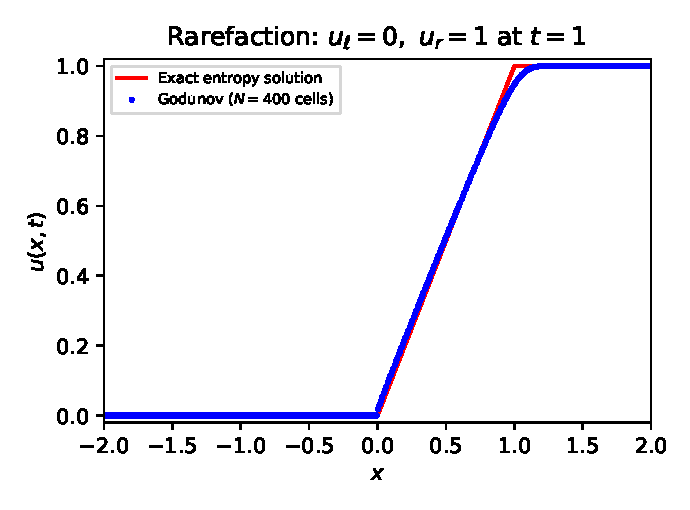
\includegraphics[width=0.44\textwidth]{figures/godunov_rarefaction.pdf}
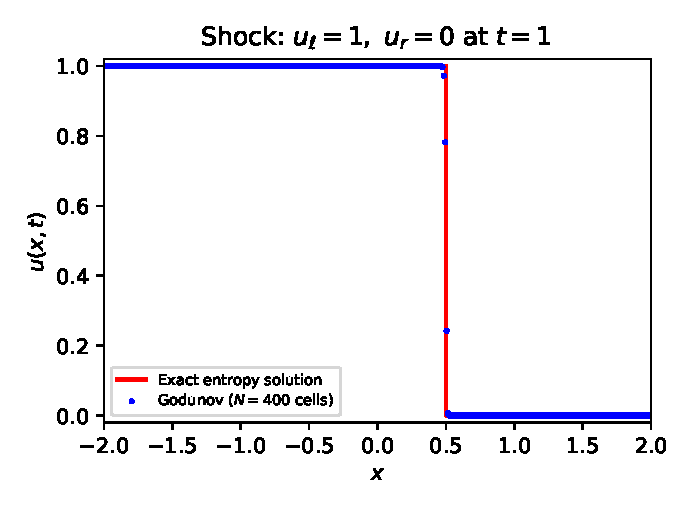
\includegraphics[width=0.44\textwidth]{figures/godunov_shock.pdf}
\caption{Godunov scheme (dots, $N=400$) against the exact entropy solution
(solid) at $t=1$. Left: rarefaction data $(0,1)$. Right: shock data
$(1,0)$. Code: \cite{code}.}
\label{fig:godunov-results}
\end{figure}

\begin{table}[htbp]
\centering
\begin{tabular}{r r r r r r}
  $N$ & $\Delta x$ & $L^1$ (rarefaction) & order & $L^1$ (shock) & order \\\hline
  200  & $2.0\times10^{-2}$ & $3.05\times10^{-2}$ & --- & $9.91\times10^{-3}$ & --- \\
  400  & $1.0\times10^{-2}$ & $1.82\times10^{-2}$ & 0.74 & $4.98\times10^{-3}$ & 0.99 \\
  800  & $5.0\times10^{-3}$ & $1.07\times10^{-2}$ & 0.77 & $2.50\times10^{-3}$ & 0.99 \\
  1600 & $2.5\times10^{-3}$ & $6.14\times10^{-3}$ & 0.80 & $1.24\times10^{-3}$ & 1.01 \\
  3200 & $1.25\times10^{-3}$ & $3.48\times10^{-3}$ & 0.82 & $6.23\times10^{-4}$ & 0.99 \\
  6400 & $6.25\times10^{-4}$ & $1.95\times10^{-3}$ & 0.84 & $3.13\times10^{-4}$ & 0.99
\end{tabular}
\caption{$L^1$ errors at $t=1$ and observed orders $\log_2(e_{N/2}/e_N)$.
All $N$ are multiples of $8$, so the shock lies on a cell interface. Code: \cite{code}.}
\label{tab:godunov-conv}
\end{table}

\paragraph{Shock.} Here $E/\Delta x$ is the shock error measured in cell widths, so a value $c$ means the
computed profile differs from the sharp shock by an amount equal to $c$ cells'
worth of mass. The shock $x=st=0.5$ lies on a cell interface iff $8\mid N$, which
matters because otherwise the cell containing it holds a mixed initial average and
the initial error depends on where the discontinuity falls inside that cell;
for such $N$ the ratio $E/\Delta x$ lies between $0.495$ and $0.501$ and the
observed order is $\approx1$ (Table~\ref{tab:godunov-conv}). On misaligned grids
($N=97,\dots,103$) it ranges from $0.55\,\Delta x$ to $0.66\,\Delta x$, so orders
computed between misaligned and aligned resolutions are unreliable (from $N=100$ to
$200$ one would obtain $1.40$); this is why the table uses $N=200\cdot2^k$.

\paragraph{Rarefaction.} The observed orders $0.74,0.77,0.80,0.82,0.84$ are still
increasing, so these experiments do not establish a first-order rate. In fact
$E/\Delta x$ grows by $0.30$ to $0.34$ per halving of $\Delta x$, roughly linearly in
$\ln(1/\Delta x)$, which is consistent with, but does not prove, an error of the form
$\Delta x\,(c+c'\ln(1/\Delta x))$, that is, first order up to a logarithm. The error is
concentrated near the fan but not at its corners: the fan interior $0.2<x<0.8$
carries about a third of it, so the rate has not stabilised.

\subsubsection{Numerical diffusion as vanishing viscosity}
\label{subsubsec:numerical-viscosity}

For the shock data the scheme is monotone, so by the discrete maximum principle
all states remain in $[0,1]$. All characteristic speeds are then nonnegative, so
the Godunov flux is the upwind flux $f(U_j^n)$, and the scheme reads
$U_j^{n+1}=U_j^n-\lambda(f(U_j^n)-f(U_{j-1}^n))$, $\lambda=\Delta t/\Delta x$.
The mechanism is that upwinding averages information from one side, and the leading
error of such an average is a diffusion term. Taylor expansion gives the modified equation
\begin{equation}
  \label{eq:modified-equation}
  u_t+u\,u_x=\frac{\Delta x}{2}\big(u(1-\lambda u)\,u_x\big)_x+O(\Delta x^2),
\end{equation}
a Burgers-type equation in conservative form, with state-dependent viscosity
$\nu(u)=\tfrac{\Delta x}2u(1-\lambda u)$, nonnegative exactly under
\eqref{eq:cfl}. In the scaled variable $\eta=(x-t/2)/\Delta x$, its travelling shock $1\to0$ of
speed $\tfrac12$ satisfies $\tfrac12u(1-\lambda u)u_\eta=\tfrac12u(u-1)$, that is,
\begin{equation}
  \frac{du}{d\eta}=\frac{u-1}{1-\lambda u},\qquad
  \eta(u)=\eta_0+(1-\lambda)\ln(1-u)-\lambda u .
\end{equation}
The profile decays exponentially to $1$ as $\eta\to-\infty$ and reaches $0$ at
a finite $\eta_0$, which conservation of mass fixes as $\eta_0=1-\lambda/2$. The
$L^1$ distance from the sharp shock is then
\begin{equation}
  \frac{\|u-u_{\rm exact}\|_{L^1}}{\Delta x}
  =2\int_0^{u_0}\frac{u(1-\lambda u)}{1-u}\,du,\qquad
  (1-\lambda)\ln(1-u_0)-\lambda u_0=-\Big(1-\frac\lambda2\Big).
\end{equation}
Table~\ref{tab:numerical-viscosity} compares this with the measured shock error on
aligned grids, where $\lambda$ equals the CFL number since $\max|U|=1$
(\texttt{numerical\_viscosity.py} \cite{code}).

\begin{table}[htbp]
\centering
\begin{tabular}{c c c c}
  CFL $=\lambda$ & measured ($N=1600$) & predicted & (pred.$-$meas.)/meas. \\\hline
  0.10 & 0.626 & 0.686 & $+9.4\%$ \\
  0.45 & 0.496 & 0.511 & $+3.1\%$ \\
  0.80 & 0.352 & 0.342 & $-3.0\%$ \\
  0.95 & 0.300 & 0.272 & $-9.3\%$
\end{tabular}
\caption{Shock $L^1$ error divided by $\Delta x$: measured (grids with $8\mid N$)
against the modified-equation prediction (code: \cite{code}).}
\label{tab:numerical-viscosity}
\end{table}

The prediction is within $10\%$ throughout (the CFL $0.95$ value is not yet
asymptotic: $0.334$ at $N=400$). Equating the error with $4\ln2\,\nu_{\rm eff}$
(Proposition~\ref{prop:viscous-profile}, $s=\tfrac12$, $\Delta=1$) defines an
effective viscosity: the measured $0.50\,\Delta x$ gives
$\nu_{\rm eff}\approx0.179\,\Delta x$ and the modified-equation profile gives
$0.184\,\Delta x$, so the effective viscosity vanishes with the mesh, the numerical
analogue of the mechanism behind Theorem~\ref{thm:vanishing-viscosity}. That theorem
concerns constant physical viscosity and does not itself give convergence of the
scheme, whose modified equation is degenerate; convergence is the content of
Theorem~\ref{thm:godunov-convergence}. The agreement of constants is empirical
evidence for the modified equation, not a proof: since
\eqref{eq:modified-equation} presupposes controlled derivatives that grow under
refinement inside a layer of width $O(\Delta x)$, the expansion is formal there, and
the sign change of the discrepancy across CFL numbers shows the agreement is only
approximate.

\subsubsection{A consistent scheme that selects the wrong solution}
\label{subsubsec:non-entropy}

Consider the flux $\widehat f_{j+1/2}=f(U_j)$ if $\tfrac12(U_j+U_{j+1})>0$ and
$f(U_{j+1})$ otherwise, which is consistent and conservative but not monotone.
For the Riemann data $U_j=-1$ ($j\le0$), $U_j=+1$ ($j>0$) every numerical flux
equals $f(\pm1)=\tfrac12$, so $U^{n+1}=U^n$ exactly and the scheme returns the
stationary upward jump, the analogue for these data of $u_A$ in
Section~\ref{sec:nonuniqueness} (a weak solution by
\eqref{eq:rankine-hugoniot-burgers} with speed $0$, but not an entropy solution).
Godunov's flux at the same interface is $f(0)=0$, and the resulting scheme
produces instead the fan $u=x/t$ of Theorem~\ref{thm:riemann-solution}. At $t=1$ the $L^1(-2,2)$
distance to the entropy solution is $1.000$ for the non-monotone scheme for all
$N=200,400,800$, since $\int|\operatorname{sgn}x-\operatorname{clip}(x,-1,1)|\,dx=1$, while for
Godunov's scheme it is $6.1\times10^{-2}$, $3.6\times10^{-2}$,
$2.1\times10^{-2}$. By the Lax--Wendroff theorem \cite[Ch.~12]{leveque2002}, if the approximations
of a consistent conservative scheme remain bounded and converge a.e.\ (or in
$L^1_{\rm loc}$), the limit is a weak solution, so consistency and conservation
alone do not select the entropy solution. Monotonicity
(Theorem~\ref{thm:godunov-convergence}) is a sufficient condition for convergence
to it, though not a necessary one for every scheme.